\documentclass[13pt]{beamer}
%teleprompter Schalter
%\setbeameroption{show notes} %un-comment to see the notes

\mode<presentation> {
	
	% The Beamer class comes with a number of default slide themes
	% which change the colors and layouts of slides. Below this is a list
	% of all the themes, uncomment each in turn to see what they look like.
	
	%\usetheme{default}
	%\usetheme{AnnArbor}
	%\usetheme{Antibes}
	%\usetheme{Bergen}
%	\usetheme{Berkeley}
	\usetheme{Berlin}
	%\usetheme{Boadilla}
	%\usetheme{CambridgeUS}
	%\usetheme{Copenhagen}
	%\usetheme{Darmstadt}
	%\usetheme{Dresden}
%	\usetheme{Frankfurt}
	%\usetheme{Goettingen}
	%\usetheme{Hannover}
	%\usetheme{Ilmenau}
	%\usetheme{JuanLesPins}
	%\usetheme{Luebeck}
%	\usetheme{Madrid}
	%\usetheme{Malmoe}
	%\usetheme{Marburg}
	%\usetheme{Montpellier}
	%\usetheme{PaloAlto}
	%\usetheme{Pittsburgh}
	%\usetheme{Rochester}
	%\usetheme{Singapore}
	%\usetheme{Szeged}
	%\usetheme{Warsaw}
	
	% As well as themes, the Beamer class has a number of color themes
	% for any slide theme. Uncomment each of these in turn to see how it
	% changes the colors of your current slide theme.
	
	%\usecolortheme{albatross}
	%\usecolortheme{beaver}
	%\usecolortheme{beetle}
	%\usecolortheme{crane}
	%\usecolortheme{dolphin}
	%\usecolortheme{dove}
	%\usecolortheme{fly}
	%\usecolortheme{lily}
	%\usecolortheme{orchid}
	%\usecolortheme{rose}
	%\usecolortheme{seagull}
	%\usecolortheme{seahorse}
	%\usecolortheme{whale}
	%\usecolortheme{wolverine}
	
	%\setbeamertemplate{footline} % To remove the footer line in all slides uncomment this line
	%\setbeamertemplate{footline}[page number] % To replace the footer line in all slides with a simple slide count uncomment this line
	
	%\setbeamertemplate{navigation symbols}{} % To remove the navigation symbols from the bottom of all slides uncomment this line
}

\usepackage[latin1]{inputenc}
\usepackage[ngerman]{babel}

% Hochschule Emden/Leer Layout einbinden
\usetheme{-hs-emden-theme}

% Hochschule Emden/Leer Hintergrundbild einbinden
\usebackgroundtemplate{
\includegraphics[width=\paperwidth]{logo/hintergrund.eps}}

% F�r Grafiken
\usepackage{float}
\usepackage{graphicx}

% F�r Code Zeigen
\usepackage{listings}
\lstset{ % Python style for highlighting
	language=Python,
	basicstyle=\small,
	otherkeywords={self},             % Add keywords here
	keywordstyle=\color{deepblue},
	emph={MyClass,__init__},          % Custom highlighting
	emphstyle=\color{deepred},    % Custom highlighting style
	stringstyle=\color{deepgreen},
	numbers=left,
	stepnumber=1,                         % Any extra options here
	showstringspaces=false            %
}
% F�r Farbe von Fonts
\usepackage{color}
\usepackage{xcolor}

% Farbe f�r Python Code
\definecolor{deepblue}{rgb}{0,0,0.5}
\definecolor{deepred}{rgb}{0.6,0,0}
\definecolor{deepgreen}{rgb}{0,0.5,0}
\definecolor{lightgray}{rgb}{.9,.9,.9}
\definecolor{darkgray}{rgb}{.4,.4,.4}
\definecolor{purple}{rgb}{0.65,  0.12,  0.82}

% Fonts for Python code, default  fixed  font  does  not  support  bold  face
\DeclareFixedFont{\ttb}{T1}{txtt}{bx}{n}{12}  %  for  bold
\DeclareFixedFont{\ttm}{T1}{txtt}{m}{n}{12}    %  for  normal

% Nummerierung f�r die Gliederung aktivieren
\setbeamertemplate{section in toc}[sections numbered]

% Dokumentinformationen
\author{Y. Mao, A. Walter und T. Quindt}
\title{ISIN}
\subtitle{Recht und Datenschutz}
%\logo{
\includegraphics[width=0.1\paperwidth]{logo/technik.eps}}
\institute{Hochschule Emden/Leer}
\date{\today}
\subject{Rechts und Datenschutz}

\AtBeginSection[]{
	\begin{frame}
		\vfill
		\centering
		\begin{beamercolorbox}[sep=8pt,center,shadow=true,rounded=true]{title}
			\usebeamerfont{title}\insertsectionhead\par%
		\end{beamercolorbox}
		\vfill
	\end{frame}
}

\begin{document}
	% Titelslide
	\begin{frame}[plain]
		\maketitle
		\centering
		\begin{figure}[H]
			
\includegraphics[width=0.3\linewidth]{logo/technik}
		\end{figure}
		\tiny{made with \LaTeX}
	\end{frame}

	% Gliederung
	\begin{frame}{Gliederung}
		\setcounter{tocdepth}{1}
		\tableofcontents
	\end{frame}
	
	\section{Einleitung}
	\subsection{Einf�hrung in Pr�fziffernsysteme}
	\begin{frame}{Einf�hrung in Pr�fziffernsysteme}
		\begin{itemize}
		\item Was sind Nummernsysteme?
		\item Wozu dienen Nummernsysteme?
		\item Wie setzen sich Identifikationsnummern zusammen?
		\item Wozu dienen Pr�fziffern?
		\item Beispiele?
		\end{itemize}

	\end{frame}
	\begin{frame}{Parit�tsbit}
		\begin{figure}[H]
			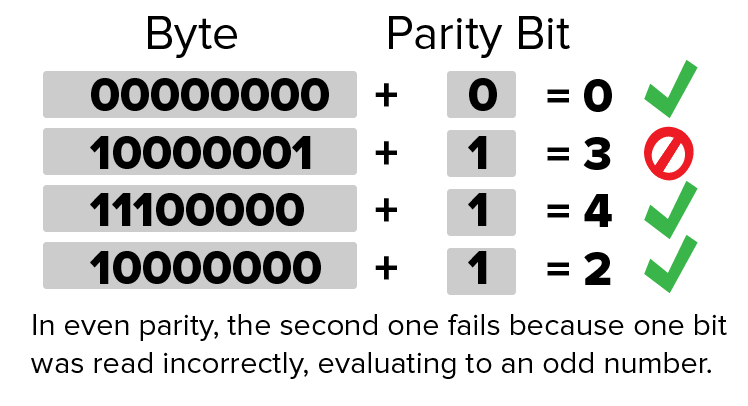
\includegraphics[width=0.9\linewidth]{Grafiken/panity_transparent.png}
			\caption{Parit�tsbit}
		\end{figure}
	\end{frame}

	\subsection{Grundlagen}
 	\begin{frame}{Grundlagen}
 	\begin{itemize}
 		\item Was sind Wertpapiere?
 		\begin{figure}[h]
 				 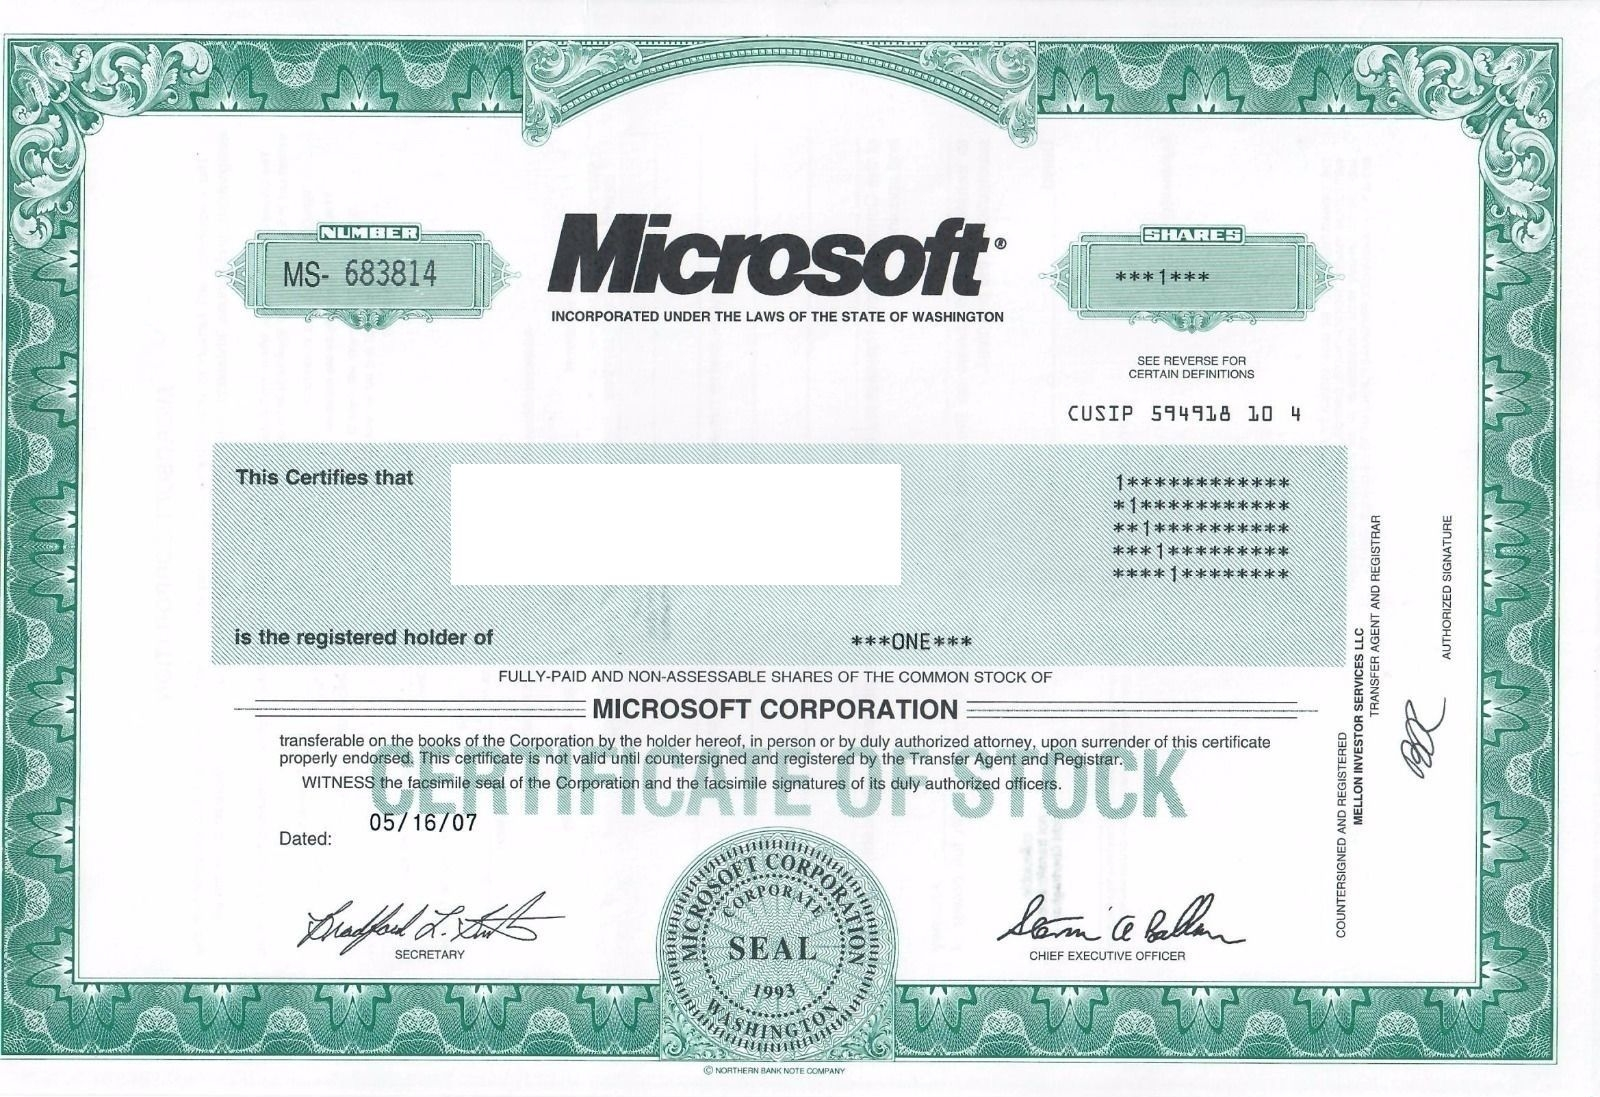
\includegraphics[width=0.45\linewidth]{Grafiken/ms-wertpapier.jpg}
 				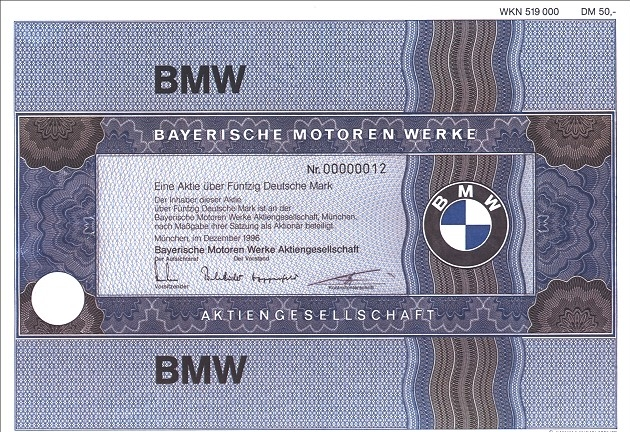
\includegraphics[width=0.45\linewidth]{Grafiken/bmw-wertpapier.jpg}
 				\caption{Beispiele f�r Wertpapiere}
 		\end{figure}
 	\end{itemize}
 	\end{frame}
 
 
 	\subsection{Historie von ISIN}
	\begin{frame}{Historie}
		
		\begin{itemize}
			\item Erste Aktie aus dem Jahr 1288
		\end{itemize}
		\begin{figure}[h]
			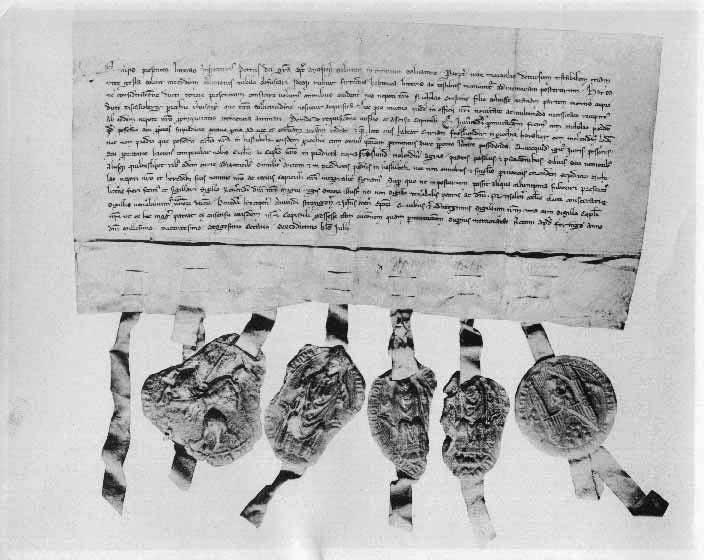
\includegraphics[width=0.5\linewidth]{Grafiken/erste-aktie.jpg}
			\caption{Aktie der Stora Kopparberg Kupfermine}
		\end{figure}
	\end{frame}
		\begin{frame}{Vorg�nger - NSIN}
		NSIN (National Securities Identifying Number)
			\begin{itemize}
				\item Deutsche NSIN 
				\\ $\rightarrow$ WKN (Wertpapierkennnummer)
				\\ $\rightarrow$  In Deutschland in 1955 eingef�hrt wurde
				\\ $\rightarrow$  besteht aus 6 Ziffern und Buchstaben
				\\ $\rightarrow$ z.B. Bayer AG mit \textbf{BAY001}
				\item US-Amerikanische NSIN 
				\\ $\rightarrow$ CUSIP (Committee on Uniform Security Identification Procedures)
				\\ $\rightarrow$  In Amerika in 1965 eingef�hrt wurde
				\\ $\rightarrow$  besteht aus 9 Ziffern und Buchstaben
				\\ $\rightarrow$ z.B. Google \textbf{38259P508}
			\end{itemize}
		\end{frame}

	\begin{frame}{Heutiger Standard - ISIN}
	ISIN (Internaltional Securities Identification Number)
	\begin{figure}[H]
		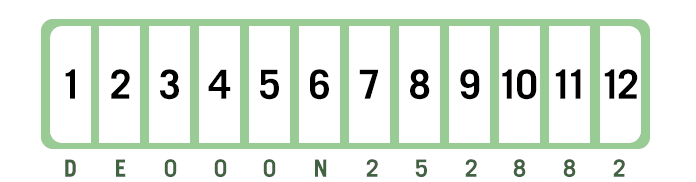
\includegraphics[width=0.9\linewidth]{Grafiken/ISIN_example.png}
		\caption{Beispiel ISIN}
	\end{figure}
	\end{frame}
	
	\section{Mathematisches Konzept}
	\subsection{ISIN Aufbau}
	\begin{frame}{ISIN Aufbau}
	\begin{figure}[H]
	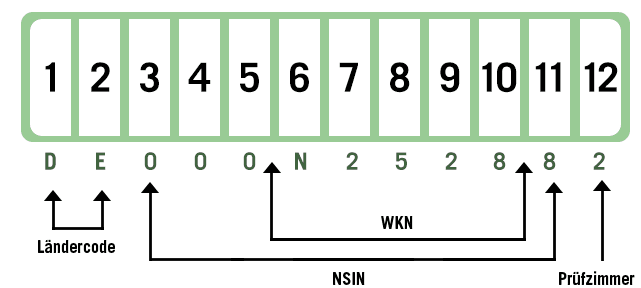
\includegraphics[width=0.85\linewidth]{Grafiken/ISIN_architectur.png}
	\caption{Aufbau einer ISIN}	
	\end{figure}
	\end{frame}
	\subsection{Pr�fziffern Berechnung}
	\begin{frame}{Pr�fziffern Berechnung}
		Auf Basis von:
		\begin{itemize}
			\item Quersummen
			\item Modularoperationen
			\item Multiplikationen
		\end{itemize}
	\end{frame}
	\begin{frame}{Pr�fziffern Berechnung}
		\begin{figure}[H]
			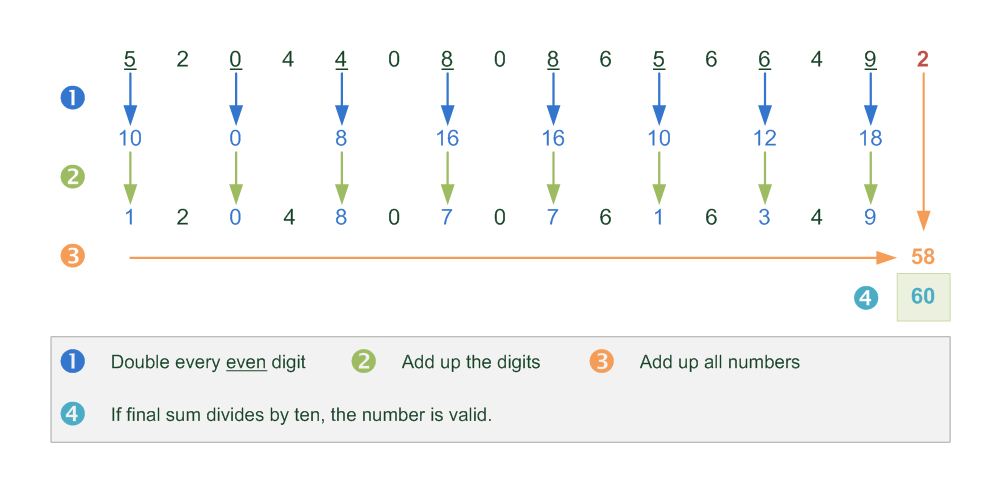
\includegraphics[width=\linewidth]{Grafiken/luhn_algorithm1.png}
			\caption{Aufbau einer ISIN}	
		\end{figure}
	\end{frame}
	\subsection{ISIN �berpr�fung}
	\begin{frame}{ISIN �berpr�fung}
	\begin{figure}[H]
		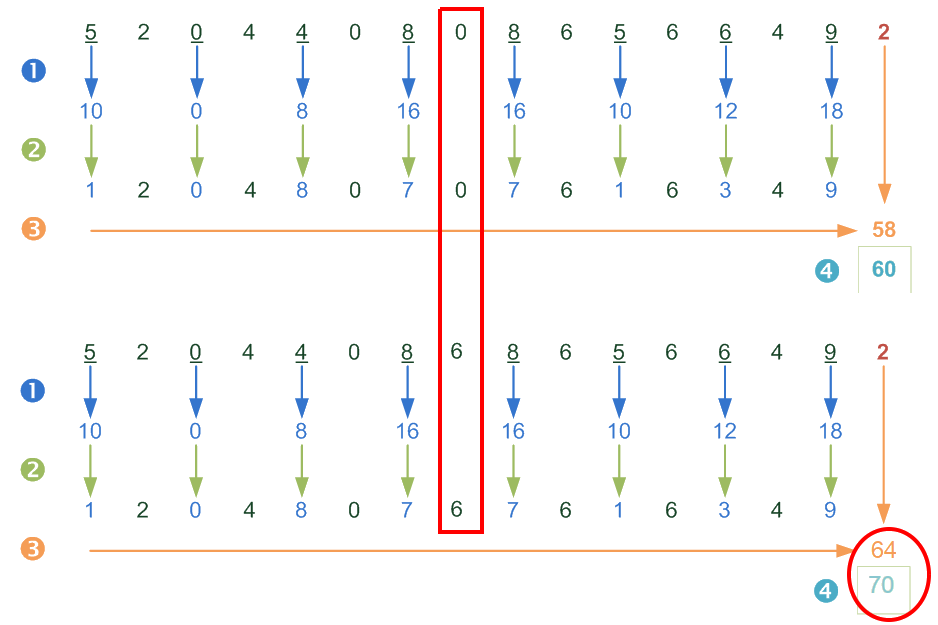
\includegraphics[width=0.9\linewidth]{Grafiken/luhn_algorithm_check_1.png}
%		\caption{Aufbau einer ISIN}	
	\end{figure}
	\end{frame}

	\subsection{Sicherheit}
	\begin{frame}{Sicherheit}
		\begin{itemize}
			\item Spezifische Permutation
			\\	$\rightarrow$ Vertauschung von Zahlen an bestimmten Stellen
			\item Zwillingsfehler(twin error)
			\\ $\rightarrow$ Vertauschung bestimmter doppelter Zahlenfolge mit anderen(44 mit 77, 33 mit 66, 22 mit 55)
			\item $\rightarrow$ Kollisionswahrscheinlichkeit
		\end{itemize}
	\end{frame}
	\begin{frame}{Spezifische Permutation}
	\begin{figure}[H]
	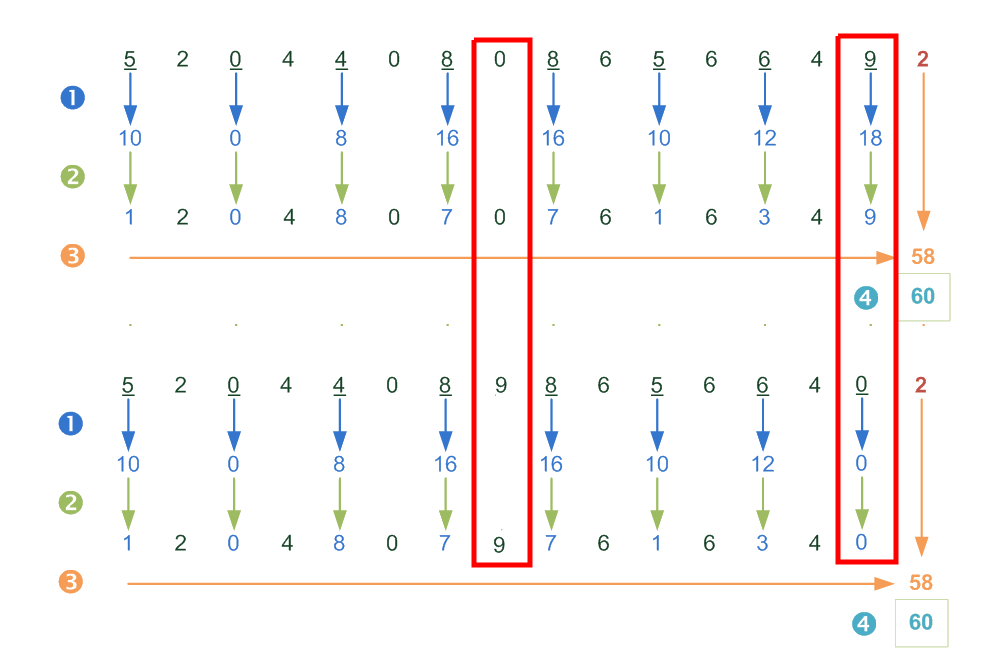
\includegraphics[width=0.9\linewidth]{Grafiken/luhn_algorithm_sicherheit_1.png}
	%		\caption{Aufbau einer ISIN}	
	\end{figure}
	\end{frame}
		
	\section{Praxis}
	\subsection{�bungen}
	\begin{frame}{�bungen}
		Bitte vervollst�ndigen Sie die folgenden ISIN mit entsprechenden Pr�fziffer.
		\begin{itemize}
			\item DE000581005\underline{\hspace{3mm}} (D=13, E=14)
			\item CH003124012\underline{\hspace{3mm}} (C=12, H=17)
			
		\end{itemize}
	\end{frame}
	
		\begin{frame}{�bungen}
	Bitte vervollst�ndigen Sie die folgenden ISIN mit entsprechenden Pr�fziffer.
	\begin{itemize}
		\item DE000581005\_ (D=13, E=14) \textcolor{red}{\textbf{5}}
		\item CH003124012\_ (C=12, H=17) \textcolor{red}{\textbf{7}}
		
	\end{itemize}
	\end{frame}
	\subsection{Code}
	\begin{frame}[fragile]{Code}
		\begin{lstlisting}
def ISIN_2_quersum(ISIN_in):

for i in range(0, len(ISIN_in)):
  quersumme = ""
  quersumme_out = 0
  if len(ISIN_in)%2 == 1:
	if i%2 == 0:
	  quersumme = quersumme + str(int(ISIN_in[i])*2)
	else:
	  quersumme = quersumme + ISIN_in[i]
  else:
    if i%2 == 1:
        quersumme = quersumme + str(int(ISIN_in[i])*2)
    else:
        quersumme = quersumme + ISIN_in[i]	

\end{lstlisting}
	
	\end{frame}
	\section{Fazit}
		\begin{frame}{Fazit}

				Nummernsysteme, welche Identifikationsnummern erzeugen, stellen f�r den Datenschutz eine entscheidenden Bedeutung dar. Manipulationen k�nnen mittels Pr�fziffern fr�hzeitig entdeckt werden. Dennoch sind diese nicht auszuschlie�en. \\
				Schlie�lich m�ssen ID-Nummern stets als sensible oder kritische Daten behandelt werden.
		
		\end{frame}
		
	% Endfolie
	\begin{frame}
		\vfill
		\centering
		\begin{beamercolorbox}[sep=8pt,center,shadow=true,rounded=true]{title}
			\usebeamerfont{title}Danke f�r die Aufmerksamkeit
		\end{beamercolorbox}
		\vfill
	\end{frame}
	\begin{frame}
		Quelle:\\
		\url{http://www.pruefziffernberechnung.de/}\\
		\url{https://en.wikipedia.org/wiki/Luhn_algorithm}\\
		\url{https://de.wikipedia.org/wiki/Internationale_Wertpapierkennnummer}
	\end{frame}
\end{document}